\chapter{Zhodnocení a budoucí kroky}\label{zhodnocení}
V této kapitole bude zhodnocena použitelnost aplikace na moment její odevzdání a navrženy vhodné budoucí kroky pro pokračování vývoje.
\section{Zhodnocení výsledné aplikace}
    Tato sekce je věnovaná zhodnocení použitelnosti výsledného návrhu a implementace aplikace. 
    \subsection{Implementace}
        Výsledná implementace aplikace obsahuje všechny potřebné funkce pro správné fungování, a také byly splněny všechny požadavky frontendového týmu ohledně úprav návrhu (viz kapitolu \ref{chapter:analyza}). Také byla přidána podpora dodatečných požadavku pro následné propojení Android aplikace a serverového backendu (viz kapitolu \ref{chapter:navrh}). Výsledný stav API byl kontrolován autorem frontendové částí aplikace -- Martinem Beranem.
        Provedená implementace v rámci této bakalářské práce je prodloužením již existující implementace. Proto pro provedené implementace s již existující implementací byla provedená analýza na základě počtu řádek kódu aplikace. Na obrázku \ref{image:code-count-main} je zobrazeny výsledky analýzy. 
        Pro analýzu byla uvažována jenom složka \enquote{be-springboot/src/main}. Stejná analýza byla provedena přes začátkem práci pro jíž existující implementaci, která byla popsána v sekci \ref{analyza:soucasnaImplementace}.
        \begin{figure}\centering
        	   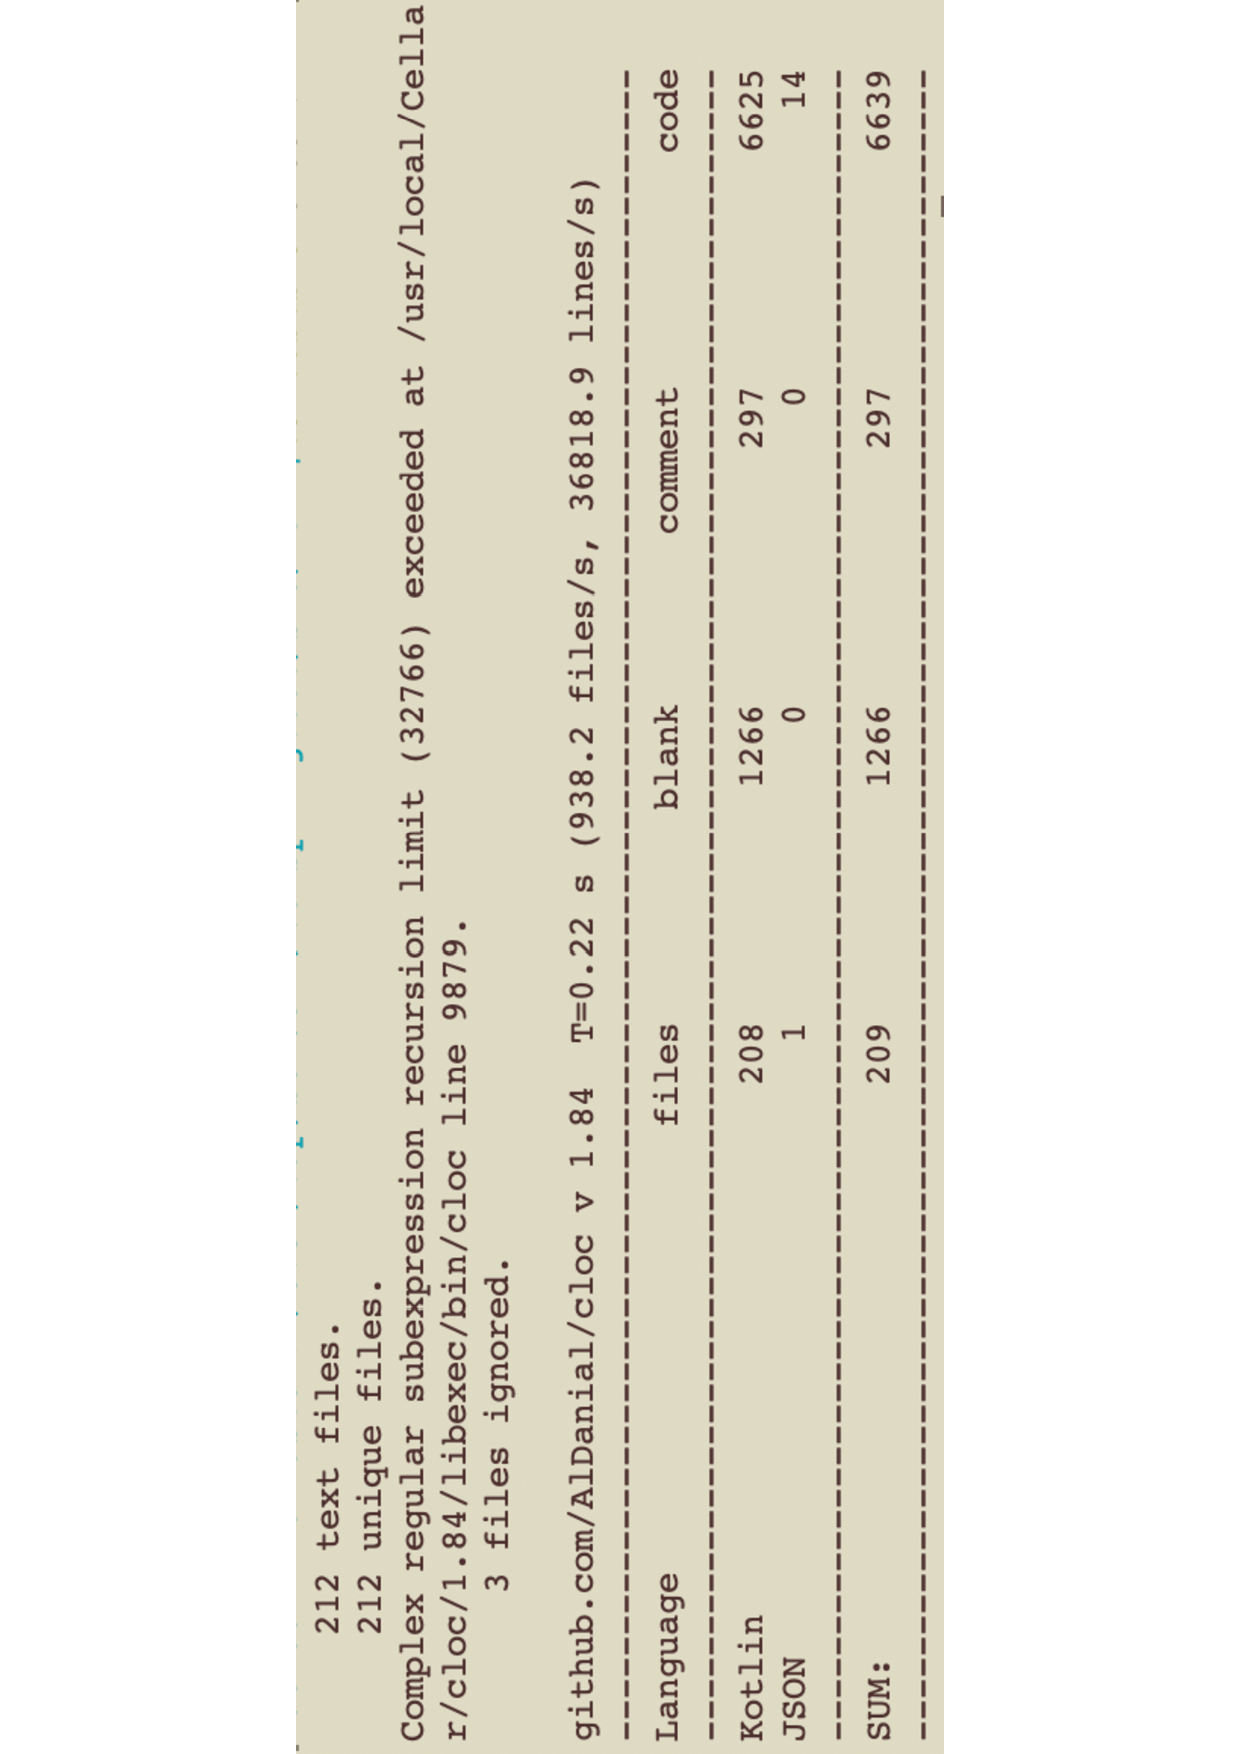
\includegraphics[angle=-90, width=0.8\textwidth]{pdfs/CodeAmountImpl2}
        	   \caption[Analýza kódu implementace]{Analýza rozsahu provedené za účelem implementace programu práci}\label{image:code-count-main}
        \end{figure}
        
        Současná implementace aplikace je funkční a je aktuálně dostupná na adrese \enquote{https://37.46.80.230/8778}. Proces nasázení aplikace byl podrobně popsán v sekci \ref{analyza:ci}. Dokumentace API aplikace je dostupná online na adrese \enquote{https://37.46.80.230/8778/swagger-ui.html}. Výsledná verze aplikace je uložena do větve \verb|dev| v rámci GitLab.
        Verze aplikace uložena do větve \verb|master| není aktuální, protože současná aplikace ještě není kompletně připravená pro fungování v produkci.
        
        Pro spuštění aplikace pomoci příkazové řádky je nutné zadat příkaz \enquote{./gradlew bootRun} v kořenové složce. Další informace o podporovaných příkazech je uvedená v souboru \enquote{README.md}, který se také nachází v kořenové složce. 
        
    \subsection{Testování}
        \begin{figure}\centering
    	   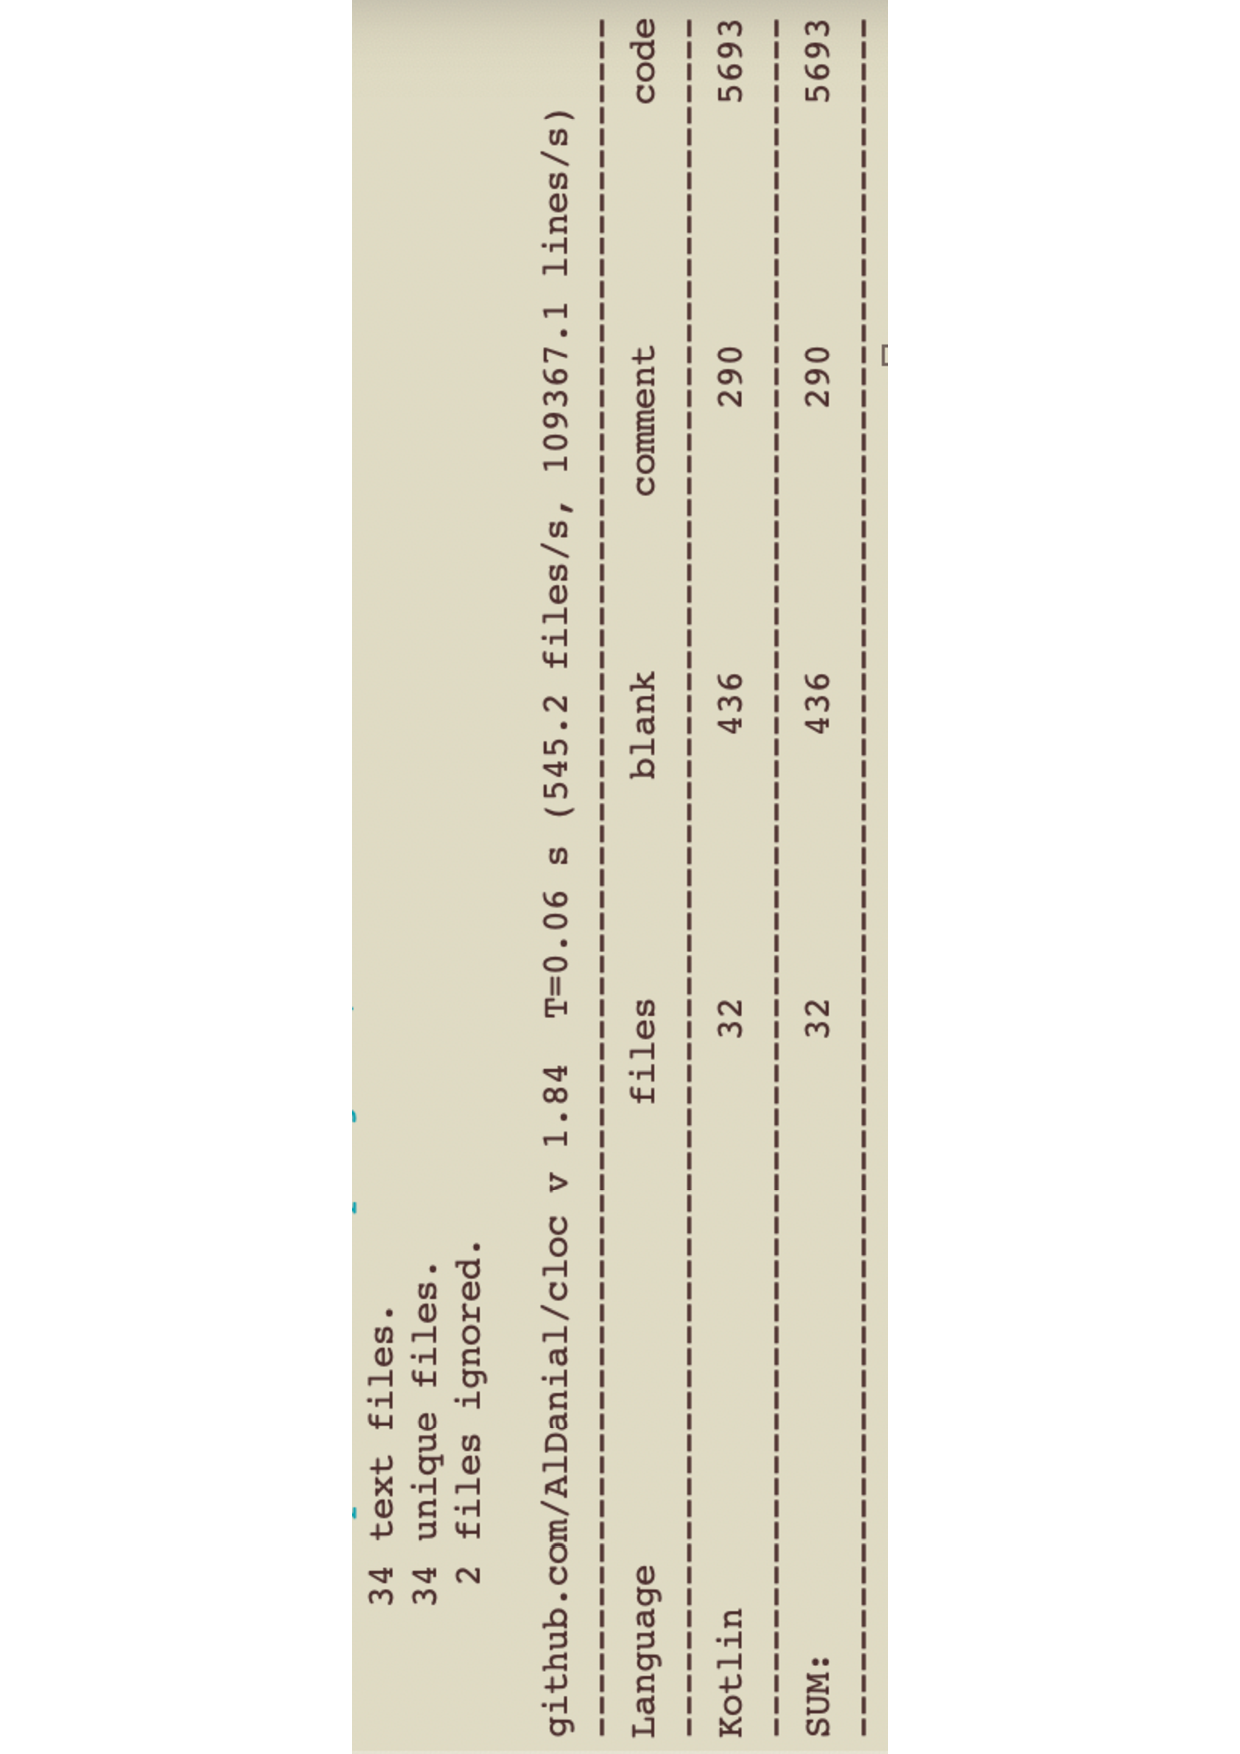
\includegraphics[angle=-90, width=0.8\textwidth]{pdfs/CodeAmountTests2}
    	   \caption[Analýza kódu testů]{Analýza rozsahu provedené za účelem testování práci}\label{image:code-count-test}
        \end{figure}
        Aplikace byla vhodně protestována pomocí unit testů a integračních testů (viz kapitolu \ref{chapter:testovani}). Analýza řádek kódů testování je zobrazena na obrázku \ref{image:code-count-test}. Pro spuštění testů pomoci příkazové řádky je potřeba zadat příkaz \enquote{./gradlew test} v kořenové složce aplikace. Proces běhu testů vyžaduje specifické nastavenou databázi PostgresSQL.
        Podrobný popis požadované konfigurace bude uveden v souboru \enquote{README.md}, který se také nachází v kořenové složce.
    \subsection{Bezpečnost}
        Předchozí verze aplikace obsahovala jenom návrh bezpečnosti pomoci přisvojení každému uživateli určitých roli v rámci rodin. Tento návrh byl následně implementován a rozšířen. Proces zjištění roli uživatele vyžadoval implementaci procesu autorizace, proto byl požit protokol OAuth 2.0. Pro zaručení bezpečné komunikace mezi klientem a serverem byl také nahrazen protokol HTTP protokolem HTTPS.
        
        V současné implementaci autorizační server je součástí serverového backendu a odpovídá, jak za registraci uživatele, tak i za přihlášení. Pro registraci uživatel má poslat dto se svými údaje na příslušný řadič\footnote{řadič je namapován na cestu \enquote{/api/v1/aut}}. Pro přistup do zmíněného řadiče se používá typ přístupu \textit{user credentials}. Uživatel potřebuje uvést adresu pro obdržení průkazů (\textit{token}), identifikátor uživatele a tajemství. Potom uživatel obdrží průkaz umožňující provést registraci.
        Pro přihlašování uživatele se používá typ obdržení průkazů \textit{resource owner password credetials}, kde uživatel potřebuje, navíc od předchozího typu, poslat svoje uživatelské jméno a heslo. Potom uživatel obdrží \textit{access token}\footnote{tento průkaz klient používá pro komunikaci se serverem} a \textit{refresh token}\footnote{tento průkaz klient používá pro obnovení \textit{access token} po vypršení jeho platnosti} jako návratové hodnoty. Platnost průkazu pro komunikaci je omezen jednou hodinou. Platnost průkazu pro obnovení průkazu pro komunikaci je omezen jedním týdnem.
        
    \section{Požadavky na změny}
        Pro zaručení správného návrhu API je potřeba propojit výsledný návrh serverového backendu a Android aplikace, která se řeší v rámci souběžné bakalářské práci. Proto je potřeba v rámci této bakalářské práci připravit API, které by bylo použitelné. Současný návrh Android aplikaci nepodporuje požadavky. Za účelem vyvarování kolizí výsledná implementace API serveru také nepodporuje požadavky na změny.

\section{Návrh budoucích kroků}
    Tato sekce je věnovaná návrhu vhodných budoucích kroků pro pokračování vývoje aplikace.
    
    \subsection{Testování}
        Výsledný stav aplikace je připravena k použiti současným stavem fronendové častí aplikace. API serveru bylo kontrolováno autorem souběžně vyvíjející se frontedové částí aplikace. Pro následující proces vývoje, nastavení Android aplikace mají být upraveny pro použití externího serveru. Po udělaných úpravách má být provedené podrobné testování jestli všechny funkce jsou implementovány správně a případně opraveny.
    
    \subsection{Implementace}
        Po úspěšném propojení serverového backendu a souběžně vybíjející Android aplikace, má být dokončená implementace chybějících funkcí. Do takových funkcí patří požadavky na změny v rámci rodiny. 
        
    \subsection{Bezpečnost}
        V současné implementaci aplikace autorizační server je součástí serverového backendu. Proto, pro zvýšení bezpečnosti aplikace, je nutné přidat možnost přihlašování pomoci externího autorizačního serveru. Proces přihlašování se potom změní následujícím způsobem. Klient se přihlásí do autorizačního serveru a obdrží \textit{access token} a \textit{refresh token}. 
        Tyhle průkazy klient potom může použit pro komunikace se serverem. Server bude ověřovat platnost průkazů dotazováním na externí autorizační server.
